\documentclass[tikz, border=5mm]{standalone}
\usepackage{amsmath}
\usetikzlibrary{arrows.meta, calc, 3d}

\begin{document}
	
	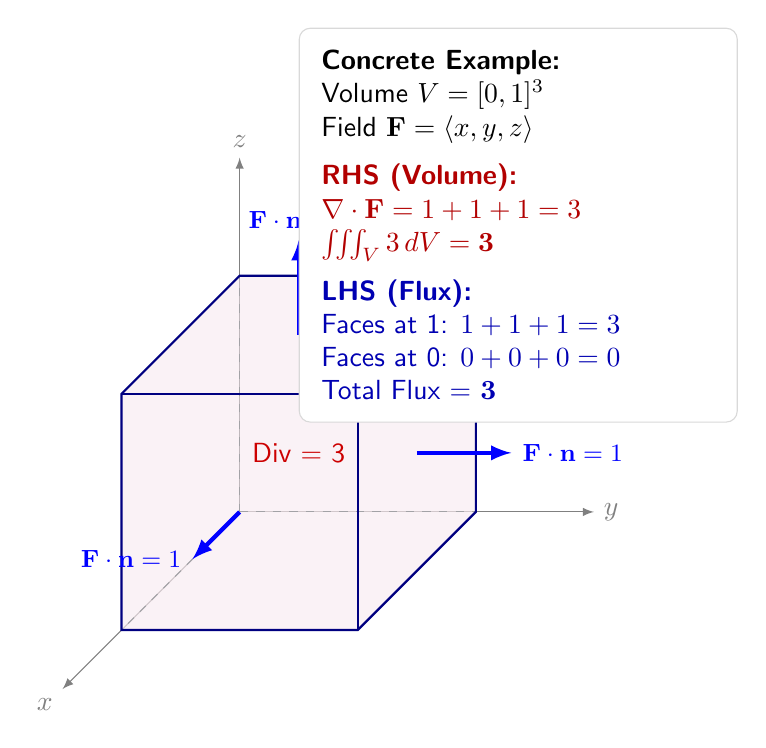
\begin{tikzpicture}[
		x={(-0.5cm,-0.5cm)}, y={(1cm,0cm)}, z={(0cm,1cm)}, % Standard isometric view
		scale=3,
		font=\sffamily,
		>=latex
		]
		
		% --- 1. Define Coordinates for Unit Cube ---
		\coordinate (O) at (0,0,0);
		\coordinate (A) at (1,0,0); % x axis corner
		\coordinate (B) at (0,1,0); % y axis corner
		\coordinate (C) at (0,0,1); % z axis corner
		\coordinate (AB) at (1,1,0);
		\coordinate (AC) at (1,0,1);
		\coordinate (BC) at (0,1,1);
		\coordinate (ABC) at (1,1,1);
		
		% --- 2. Draw Axes (Background) ---
		\draw[->, gray, thin] (O) -- (1.5,0,0) node[below left] {$x$};
		\draw[->, gray, thin] (O) -- (0,1.5,0) node[right] {$y$};
		\draw[->, gray, thin] (O) -- (0,0,1.5) node[above] {$z$};
		
		% --- 3. Fill Volume (RHS Visualization) ---
		% Transparent red cube representing the volume V
		\fill[red!10, opacity=0.5] (O) -- (B) -- (BC) -- (C) -- cycle; % Back face
		\fill[red!10, opacity=0.5] (O) -- (A) -- (AC) -- (C) -- cycle; % Left face
		\fill[red!10, opacity=0.5] (O) -- (A) -- (AB) -- (B) -- cycle; % Bottom face
		
		% --- 4. Draw Hidden Edges ---
		\draw[dashed, gray] (O) -- (A);
		\draw[dashed, gray] (O) -- (B);
		\draw[dashed, gray] (O) -- (C);
		
		% --- 5. Draw Visible Faces and Edges ---
		% Front-Right (y=1)
		\fill[blue!5, opacity=0.3] (B) -- (AB) -- (ABC) -- (BC) -- cycle;
		% Front-Left (x=1)
		\fill[blue!5, opacity=0.3] (A) -- (AB) -- (ABC) -- (AC) -- cycle;
		% Top (z=1)
		\fill[blue!5, opacity=0.3] (C) -- (AC) -- (ABC) -- (BC) -- cycle;
		
		\draw[thick, blue!50!black] (A) -- (AB) -- (B) -- (BC) -- (C) -- (AC) -- cycle;
		\draw[thick, blue!50!black] (AB) -- (ABC);
		\draw[thick, blue!50!black] (BC) -- (ABC);
		\draw[thick, blue!50!black] (AC) -- (ABC);
		
		% --- 6. Draw Flux Vectors (LHS Visualization) ---
		% Field F = <x, y, z>
		
		% Face x=1 (Front Left): Normal (1,0,0). Center (1, 0.5, 0.5). F=(1, 0.5, 0.5). F.n = 1
		\draw[->, blue, line width=1.5pt] (1, 0.5, 0.5) -- (1.4, 0.5, 0.5) node[left] {\small $\mathbf{F}\cdot\mathbf{n}=1$};
		
		% Face y=1 (Front Right): Normal (0,1,0). Center (0.5, 1, 0.5). F=(0.5, 1, 0.5). F.n = 1
		\draw[->, blue, line width=1.5pt] (0.5, 1, 0.5) -- (0.5, 1.4, 0.5) node[right] {\small $\mathbf{F}\cdot\mathbf{n}=1$};
		
		% Face z=1 (Top): Normal (0,0,1). Center (0.5, 0.5, 1). F=(0.5, 0.5, 1). F.n = 1
		\draw[->, blue, line width=1.5pt] (0.5, 0.5, 1) -- (0.5, 0.5, 1.4) node[above] {\small $\mathbf{F}\cdot\mathbf{n}=1$};
		
		% Note: Faces at x=0, y=0, z=0 have F perpendicular to n or zero component, flux is 0.
		% We visually indicate the zero flux faces with a small text
		\node[gray, scale=0.7] at (0, 0.5, 0.5) {Flux=0};
		
		% --- 7. Explanatory Text Box ---
		\node[anchor=north west, fill=white, draw=gray!30, rounded corners, inner sep=8pt] 
		at (-0.5, 0, 1.8) {
			\begin{minipage}{5cm}
				\textbf{Concrete Example:}\\
				Volume $V=[0,1]^3$\\
				Field $\mathbf{F} = \langle x, y, z \rangle$
				
				\vspace{0.2cm}
				\color{red!70!black}
				\textbf{RHS (Volume):}\\
				$\nabla \cdot \mathbf{F} = 1 + 1 + 1 = 3$\\
				$\iiint_V 3 \, dV = \mathbf{3}$
				
				\vspace{0.2cm}
				\color{blue!70!black}
				\textbf{LHS (Flux):}\\
				Faces at 1: $1+1+1 = 3$\\
				Faces at 0: $0+0+0 = 0$\\
				Total Flux = $\mathbf{3}$
			\end{minipage}
		};
		
		% --- 8. Labels ---
		\node[red!80!black] at (0.5, 0.5, 0.5) {Div = 3};
		
	\end{tikzpicture}
	
\end{document}